% Paper 2, first full draft (2026-11-21). Not submitted.
% Every number carries a comment naming the RESULTS.md (or table/results file) it was copied from.
% Source key (full paths, all relative to the repo root):
%   BENCH = experiments/uniformity_benchmark/RESULTS.md
%   RT0   = experiments/redteam_uniformity/RESULTS.md
%   S1    = experiments/uniformity_paper/step1/RESULTS.md
%   RT1   = experiments/redteam_uniformity_step1/RESULTS.md
%   S2    = experiments/uniformity_paper/step2/RESULTS.md   (S2T = experiments/uniformity_paper/step2/table.md)
%   RT2   = experiments/redteam_uniformity_step2/RESULTS.md
%   CD    = experiments/chanhudaro_followup/RESULTS.md
%   RR    = experiments/recchia_rerun/RESULTS.md
% Comments give the full path the first time in each paragraph and the key afterwards.
\documentclass[11pt,a4paper]{article}

\usepackage[T1]{fontenc}
\usepackage[utf8]{inputenc}
\usepackage{newtxtext,newtxmath}
\usepackage[margin=2.5cm]{geometry}
\usepackage{microtype}
\usepackage{graphicx}
\usepackage{booktabs}
\usepackage{tabularx}
\usepackage{caption}
\usepackage{xcolor}
\usepackage[round,authoryear]{natbib}
\usepackage{xurl}
\usepackage[hidelinks]{hyperref}
\usepackage{setspace}

\captionsetup{font=small,labelfont=bf,labelsep=period}
\setstretch{1.08}
\graphicspath{{figures/}}

\newcommand{\sign}[1]{\textsf{#1}}

% REVISION-PENDING: title. "carry no place signal" is equivalence wording (waits on bootstrap/TOST, REVIEW_1 M3); "one sign stock" vs "one seal vocabulary" (S13) decided with it.
\title{\textbf{Two cities, one sign stock: Indus seal texts from Mohenjo-daro\\and Harappa carry no place signal beyond a within-city floor}}
% Public copy is anonymous, like docs/paper/latex/main.tex. The named copy for submission lives in the gitignored docs/paper/submission/ folder.
\author{Anonymous submission}
\date{}

\begin{document}
\maketitle

\begin{abstract}
\noindent Indus seal texts are often described as uniform across the civilisation, but to our knowledge the claim has not been tested against a calibrated within-site baseline. % REVISION-PENDING: Yadav 2013 (Scripta 5) still unread; keep "to our knowledge" until it is.
We ask whether a classifier can tell seal texts from Mohenjo-daro and Harappa apart better than it can tell apart two halves of one city.
% REVISION-PENDING: pool-level bootstrap CI and TOST at +-0.05 (REVIEW_1 M3). "It cannot." dropped; equivalence wording below waits on that analysis.
The between-city score exceeds the within-city floor by +0.005 to +0.042 AUC, and a shuffled-label null by +0.014 to +0.054, in two overlapping editions, with 98--100\% power to detect a local sign stock covering 15\% of tokens. % experiments/redteam_uniformity_step2/RESULTS.md (safe wording)
The same frozen pipeline finds place in readable seal legends.
Ur III seal impressions from Umma and Girsu exceed every structural within-city floor by +0.16 to +0.31, and Latin owner and maker marks from Britannia and Germania exceed theirs by +0.12 to +0.14. % experiments/uniformity_paper/step2/RESULTS.md (structural floors; random halves give +0.355 and +0.404)
In Ur III much of the place signal sits in personal names. % REVISION-PENDING: owner/father vs patron name split (REVIEW_1 S1)
It survives the removal of place names, gods and theophoric names (+0.09 to +0.27); once personal names are removed it still clears the Umma reign floor but no longer the strictest floor, two reigns of Girsu. % experiments/redteam_uniformity_step2/table.md (noPN rows)
Planted-name tests then bound the Indus case.
% REVISION-PENDING: finer planted-name grid r = 0, 0.35, 0.40, 0.45 with bootstrap variance (REVIEW_1 M2); the "about 30%" bound below is unchanged until then.
Site-specific names drawn from real Ur III frequencies cannot be on more than about 30\% of seals, and invented name stocks on more than 10--20\%; 99.8\% of Ur III legends carry a personal name. % experiments/redteam_uniformity_step2/table.md (A3 footnote: raw Umma + Girsu legends)
The result has limits.
Sealings and moulded tablets differ between the two cities.
Chanhu-daro is a consistent near-miss (+0.13 to +0.17, $q = 0.06$ against a bar of 0.05), partly carried by an end sign that does not occur on seals from either big city. % experiments/chanhudaro_followup/RESULTS.md
Comparisons with smaller sites are underpowered or inconclusive.
A reimplementation of \citet{recchia2016} is too weak to confirm or reject their geographic result.
Finally, a naive site classifier on Linear B tablets learns scribes rather than palaces, which shows why any site contrast needs a within-site floor.

\medskip
\noindent\textbf{Keywords:} Indus script; seals; regional variation; personal names; statistical power; within-site baseline
\end{abstract}

\section{Introduction}
\label{sec:intro}

\paragraph{The claim.} Indus sign sequences have long been described as uniform across the area of the civilisation.
\citet{parpola1994} is the standard statement of this view, as later authors cite it \citep{kenoyer2010,jamison2017}. % TODO: verify the Parpola 1994 page and wording (LITERATURE.md sec. 1 and 10: quote seen only in a search snippet). Do not quote until checked.
The closest computational test is a clustering study.
\citet[p.~19]{yadav2017} found no significant association between clusters of texts and archaeological sites; their one exception was a cluster rich in Harappa sealings.
They read this as ``a high level of uniformity of writing over the entire stretch of the Indus civilization'' \citep[pp.~20--21]{yadav2017}.
\citet{nair2026} reports that one positional statistic is similar across sites.
Neither study asks how different two cities should look if they did differ, or how different two parts of one city look when nothing separates them.
% TODO: Yadav 2013 (Scripta 5: 67-103) is directly on this question and still unread: its open copy is on harappa.com, which blocks automated clients (2026-11-21). Read by hand before submission; abstract and intro wording say "to our knowledge" until then.

\paragraph{The counter-claims.} Other authors expect regional variation.
\citet[p.~viii]{wells2015} notes ``marked regional differences in sign uses and artifact inventories'' and calls for work on regional differences in text structure.
Citing his earlier study \citep{wells2011}, he adds that ``sign inventories differ by site and artifact type'': some signs are more common at Mohenjo-daro or at Harappa, and his example, sign 400, occurs in 358 Harappa texts against 79 from Mohenjo-daro, 325 of the Harappa ones on miniature tablets \citep[p.~3]{wells2015}. % Archaeopress open sample of Wells 2015, pp. viii-ix and 3 (read 2026-11-21)
That is a raw frequency comparison in which site and object type move together; our seal-only design with a within-site floor is meant to separate them.
\citet[p.~lvi]{kenoyer2010} predicted that site-level analysis would force a revision of the uniformity assumption.
\citet[p.~219]{kenoyer2020} suggests that the script wrote names and commodities ``in many regional dialects and even different languages''.
Seal imagery and carving style do vary.
\citet{ameri2013} documents regional diversity in seal motifs, as summarised by \citet[p.~467]{petrie2018}. % TODO: Ameri 2013 not accessed directly (LITERATURE.md sec. 3); claims seen via Petrie et al. 2018: 467.
\citet{jamison2017} finds patterned variation in unicorn carving styles, in groups that cross sites.
\citet[p.~465]{petrie2018} argue that seals and sealings ``exemplify patterns of variation'' as well as uniformity.
We test texts, not imagery.
Our result concerns which signs appear on seals and in which pairs.
It says nothing about motifs, carving style or seal shape, and it does not contradict the work above.

\paragraph{The conflict.} One study reports a site signal in the texts themselves.
\citet{recchia2016} summed latent semantic analysis (LSA) vectors of inscriptions by site for five sites and report that the resulting map recovers the sites' relative positions.
We were able to read only the abstract of that paper.
We reimplemented its method from that description (Section~\ref{sec:recchia}).

\paragraph{Why a floor.} A classifier that tells two groups of texts apart has found some difference, but not necessarily the one in the labels.
Site labels are entangled with excavation area, period, object type and, in readable corpora, scribe.
A classifier can learn any of these.
This is a known problem in applied machine learning, where a model trained to find disease learned which hospital an image came from \citep{zech2018,kapoor2023}.
The remedy is a within-site floor: the same pipeline, at the same size, scoring two parts of one site.
Place signal is then the gap between the between-site score and that floor.
We also need power: a planted difference of known size, to show the test could have found one.

\paragraph{Main result.} Seal texts from Mohenjo-daro and Harappa differ no more than two halves of one city. % REVISION-PENDING: equivalence wording, bootstrap CI + TOST (REVIEW_1 M3)
In readable seal legends, much of the city signal comes through personal names.
So Indus seals cannot be carrying site-specific personal names at anything like the rate of Ur III seals: at most about 30\% of seals could carry them, against 99.8\% of Ur III legends. % experiments/redteam_uniformity_step2/RESULTS.md % REVISION-PENDING: finer planted-name grid (REVIEW_1 M2)
Section~\ref{sec:methods} describes the pipeline.
Section~\ref{sec:results} gives the three supporting results and the limits.
Section~\ref{sec:discussion} discusses what the bound means.

\section{Data}
\label{sec:data}

\paragraph{Indus.} We use the two standard editions: \citet{mahadevan1977} (M77) and the Interactive Corpus of Indus Texts \citep[ICIT;][]{icit}, which follows the sign list of \citet{wells2015}.
Corpus construction, de-duplication and the concordance between the two sign lists follow \citet{openindus2026corpus}.
That paper also measured how often the two editions disagree.
The two editions are overlapping editions of largely the same objects, not independent samples: for Mohenjo-daro and Harappa, ICIT transcribes most of the objects in M77 again from the same publications and photographs, and adds later finds.
Agreement between them shows that a result does not depend on one editor's sign list and readings; it is not a replication on new material. % REVIEW_1 B1.1 / S5; overlap count not yet made (REVISION-PENDING: M77-ICIT object overlap for MD and Harappa seals)
Seals are the primary object type, since Mohenjo-daro and Harappa inscribed different objects in different proportions \citep[p.~4]{fuls2024}.
Sealings and tablets are analysed separately.
Within Mohenjo-daro, M77 locus codes give excavation areas.
We checked them against field-number prefixes in the 1930s registers.
No M77 locus code contradicts the register field numbers it can be linked to; on the HR+VS side, 101 of 198 texts could not be confirmed. % experiments/redteam_uniformity_step1/RESULTS.md (attack 4)

\paragraph{Readable references.} We chose readable corpora of short legends on seals or labels, where sites are known.
\begin{itemize}
  \item \emph{Ur III seal legends}, Umma and Girsu: impressions from ORACC \citep{oracc}, and one entry per physical seal from CDLI \citep{cdli}.
  Within-city splits use reign, and museum collection where it stands in for archive.
  The catalogues give almost no excavation context: 16 of 13,517 Umma texts have an excavation number. % experiments/uniformity_paper/step2/RESULTS.md ("Could not do")
  Most Umma and Girsu tablets reached museums through the antiquities market in large lots, so the Ur III contrast is between-city and between-archive at once; the Indus contrast, between two excavated cities, is not. % REVIEW_1 B2.3 / S9
  \item \emph{Latin instrumentum}, owner and maker marks from Britannia and Germania, from EDH \citep{edh}.
  Within-province splits are Rhineland-Palatinate against Baden-W\"urttemberg and Hesse in Germania, and north against south in Britannia.
  \item \emph{Linear B} tablet lines from Knossos and Pylos, from DAMOS \citep{damos}, with scribal hand attributions.
  \item \emph{Old Babylonian} seal impressions from Nippur and Isin (ORACC), used only descriptively because they were underpowered. % experiments/uniformity_paper/step2/RESULTS.md
\end{itemize}
These corpora are written in words or syllables, while Indus is written in signs.
A word may carry more information than an Indus sign.
We return to this in Section~\ref{sec:limits}.
Third-party texts are not redistributed; scripts rebuild every pool from the public sources (Section~\ref{sec:availability}).

\section{Method}
\label{sec:methods}

\paragraph{One frozen classifier.} Every condition runs through the same pipeline, unchanged from an earlier site test.
Each text becomes a set of binary features: the signs (or words) it contains and the adjacent pairs within a line, kept if they occur in at least two texts. % experiments/site_signal/lib.py (design, min_df=2); code, not a RESULTS file
The two-text threshold is counted on the whole draw, test folds included; it uses no labels.
A Bernoulli naive Bayes classifier scores each text out of fold, in grouped five-fold cross-validation repeated three times. % experiments/uniformity_benchmark/run.py score() -> experiments/site_signal/lib.py oof_scores(model="nb", k=5, reps=3); code
The grouping unit keeps related texts in the same fold.
For Indus it is the text, so impressions are not grouped by seal or carver. % experiments/uniformity_paper/step2/s2.py L208, L225 (group = text id); RT1 attack 2
For the ORACC Ur III impressions it is one sealing on one tablet, so impressions of one seal on different tablets can fall in different folds; the CDLI pool, one entry per physical seal, groups by CDLI seal number, or by the composite's own P-number where none is given. % experiments/uniformity_paper/step2/build2.py L133 (group = P-number.seal), L174-178 (group = seal_id or P-number)
For Latin it is the inscription, and for Linear B the tablet. % experiments/uniformity_benchmark/build.py L149; experiments/uniformity_paper/step1/build.py L8, L147
The score is the area under the ROC curve (AUC).
An AUC of 0.5 means the two groups cannot be told apart.
Before sampling, a cleaning step drops any text string found at both sites and removes near-duplicates \citep{openindus2026corpus}.
This removes shared material from every condition alike, Indus included. % experiments/uniformity_paper/step1/RESULTS.md (caveats)
The cleaning step uses the site labels: it removes the most widely shared texts from exactly the comparison being scored.
For the Indus test this pushes towards separation, which is conservative for a null result; for the readable references it can inflate separation.
Planted stocks and names (below) are inserted after cleaning, so planted strings that happen to occur at both sites are not removed, as real ones would be. % experiments/redteam_uniformity_step2/rt2.py L505; REVIEW_1 B3.4 / S12

\paragraph{Matched size and length mix.} Each comparison draws the same number of texts per side.
For each between-site condition and its floor, that number is the smaller of the two pools' natural sizes, capped at 227 texts per side; the whole Ur III pools run at the cap. % docs/prereg/uniformity_paper_step2.md L14-15 (matched size; at most 227 per side)
Reference texts are drawn to match the length distribution of the Indus seals, because shorter texts are harder to classify.
We report the median AUC over repeated draws: 30 draws per condition in step 1 and its red team, 50 in step 2 and its red team, and 200 for the Chanhu-daro baseline. % experiments/uniformity_paper/step1/RESULTS.md; experiments/redteam_uniformity_step1/RESULTS.md; experiments/uniformity_paper/step2/RESULTS.md; experiments/redteam_uniformity_step2/RESULTS.md; experiments/chanhudaro_followup/RESULTS.md (T0)

\paragraph{Between minus within.} For each pair of sites we compute $\Delta$ = median between-site AUC $-$ median within-site AUC, at the same size.
The within-site floor is either a structural split (excavation area, reign, collection, region, scribe group) or random halves of the larger site.
A pair ``differs'' when $\Delta \geq 0.05$, the Benjamini--Hochberg $q$ against the floor is at most 0.10, and the power gate passes. % docs/prereg/uniformity_paper_step2.md (pair verdicts); margin 0.05 also in experiments/uniformity_paper/step2/RESULTS.md
A pair is ``same'' when $\Delta < 0.05$ and the gate passes. % REVISION-PENDING: "same" is a point-estimate rule, not an equivalence test; bootstrap CI + TOST (REVIEW_1 M3)
Otherwise the pre-registration calls it ``underpowered''.
That label covers two different cases, and we separate them in reporting.
A pair is \emph{underpowered} when the gate fails.
It is \emph{inconclusive} when the gate passes and $\Delta \geq 0.05$, but $q$ is above 0.10: the test could have seen a difference of that size, and the point estimate is that large, but it is not distinguishable from the floor's own spread. % REVIEW_1 B3.7

\paragraph{Shuffled-label null.} Random halves of a small pool score below 0.5. % experiments/uniformity_paper/step1/RESULTS.md (C2 note); experiments/uniformity_paper/step2/RESULTS.md
Pooled out-of-fold AUC is biased below 0.5 when there is no signal, and more so at small $n$ \citep{airola2011}; removing shared strings may add to this.
A low floor makes a between-site score look high.
The second red team therefore added a shuffled-label null for every condition: the same pool and size with site labels permuted.
It reports $\Delta_{\mathrm{null}}$ = between $-$ null median, and a conservative $\Delta_{\mathrm{cons}}$ = between $-$ the larger of the floor and the null. % docs/prereg/redteam_uniformity_step2.md; values in experiments/redteam_uniformity_step2/RESULTS.md

\paragraph{Planted stocks.} To measure power we plant a local sign stock in one site.
A share $s$ of that site's tokens is replaced by a 20-sign stock drawn from the pool's common signs.
(We write $s$ for this share, which the pre-registrations call $q$, to keep $q$ for Benjamini--Hochberg values.)
Power at $s$ is the share of planted draws whose AUC exceeds the within median by at least 0.05.
The gate requires power of at least 80\% at $s = 0.15$. % experiments/uniformity_paper/step2/RESULTS.md (Part 2 columns)
This checks power against one kind of effect, a block of signs used at one site; it says nothing about diffuse shifts in the frequency or order of shared signs. % REVIEW_1 B3.5; REVISION-PENDING: diffuse planted effect, LR and JS-divergence test (S2)
For the readable references the gate plants a stock of 100 new symbols at $s = 0.15$ with labels permuted, and counts a detection when the AUC reaches the larger of 0.65 and the null's 95th percentile. % experiments/uniformity_paper/step2/RESULTS.md (Part 1 gate)

\paragraph{Planted names.} To bound how many Indus seals could carry site-specific names, we keep the real site labels and give a share $r$ of seals at each city a local name.
Names take three forms: one new sign per name, two shared signs per name, or names spelt in shared signs with real Ur III name frequencies.
For each $r$ we record the share of draws whose gap above the floor exceeds the observed gap.
A name load is excluded when at least 95\% of draws exceed it. % experiments/redteam_uniformity_step2/table.md (A3 header) and RESULTS.md

\paragraph{Pre-registration and red teams.} Each step was written up before it was run.
The write-up and its code were hashed (SHA-256) into a timestamped file in the project repository before any condition was scored.
The timestamps are self-recorded, and each hash line was committed to the public repository together with that step's results, so a reader cannot verify from the repository alone that the hashes predate scoring. % git log -- docs/prereg/HASHES.txt: hash lines committed with results (step 2 d7ad778; RT2 + CD ae300d2; RR ecbcc0d)
After each step, a separate agent attacked the result with its own pre-registered kill rules.
Table~\ref{tab:prereg} lists the eight runs.
All of them were designed, run and scored within about one day. % commit dates 2026-11-21, docs/prereg/HASHES.txt history
The pre-registrations protected less than the word suggests.
The Mohenjo-daro--Harappa result itself (0.49 in the first benchmark, then 0.55 like-for-like) was known before every pre-registration. % experiments/uniformity_benchmark/RESULTS.md (caveats: "Only references were blind. The Indus number was known before the prereg.")
What was blind is the reference conditions, the floors and nulls for the later Indus pools, the planted tests and the red-team attacks.
One bar was also tightened after the fact: the Chanhu-daro follow-up, written after step 2 had been scored, requires $q_{\mathrm{chance}} \leq 0.05$ against the shuffled null, where the step-2 rule asked for $q_{\mathrm{floor}} \leq 0.10$ against the floor (Section~\ref{sec:limits}). % docs/prereg/chanhudaro_followup.md L31-32; docs/prereg/uniformity_paper_step2.md (pair verdicts)
Earlier steps were changed by later ones, and we report those changes.
The first benchmark compared an Indus AUC of 0.49 with reference corpora. % experiments/uniformity_benchmark/RESULTS.md
The first red team showed that this number came from a different pool and design, and that the like-for-like value was 0.55. % experiments/redteam_uniformity/RESULTS.md
The second red team showed that Linear B, used in step 1 as a positive reference, cannot be shown to carry place beyond its scribes. % experiments/redteam_uniformity_step1/RESULTS.md (0.524 with series balanced, hands held out)
The third broke the claim that name-free legends carry no place (Section~\ref{sec:names}). % experiments/redteam_uniformity_step2/RESULTS.md
The results below are the versions that survived.

\begin{table}[t]
\centering
\small
\caption{Pre-registered runs. Each tag names the rows hashed in \texttt{docs/prereg/HASHES.txt}; the timestamps there are self-recorded, and the rows became public with the results.}
\label{tab:prereg}
\begin{tabularx}{\textwidth}{lXl}
\toprule
Run & What it tested & Verdict \\
\midrule
\texttt{uniformity\_benchmark} & Indus against four reference pairs & superseded \\ % experiments/uniformity_benchmark/RESULTS.md
\texttt{redteam\_uniformity} & like-for-like Indus value; label leaks & stands weakened \\ % experiments/redteam_uniformity/RESULTS.md
\texttt{uniformity\_paper\_step1} & Linear B; name-free references; within-city floor & see red team \\ % experiments/uniformity_paper/step1/RESULTS.md
\texttt{redteam\_uniformity\_step1} & scribes, findspots, sign lists, power & broken on reference side; Indus stands \\ % experiments/redteam_uniformity_step1/RESULTS.md
\texttt{uniformity\_paper\_step2} & seal references with own floors; all-site map & whole supported; name-free refuted \\ % experiments/uniformity_paper/step2/RESULTS.md
\texttt{redteam\_uniformity\_step2} & name tagging, shuffled null, planted names & see Section~\ref{sec:results} \\ % experiments/redteam_uniformity_step2/RESULTS.md
\texttt{chanhudaro\_followup} (+\,\texttt{\_deviation1}) & Chanhu-daro: place, period, copies, signs & no robust difference \\ % experiments/chanhudaro_followup/RESULTS.md
\texttt{recchia\_rerun} & five-site geography after \citet{recchia2016} & underpowered \\ % experiments/recchia_rerun/RESULTS.md
\bottomrule
\end{tabularx}
\end{table}

\section{Results}
\label{sec:results}

% REVISION-PENDING: subsection title and first paragraph use tie / "cannot be told apart" wording; wait on pool-level bootstrap CI + TOST at +-0.05 (REVIEW_1 M3).
\subsection{Mohenjo-daro and Harappa seals tie with the floor and the null}
\label{sec:tie}

Seal texts from Mohenjo-daro and Harappa cannot be told apart by the signs they use.
Between-city AUC is 0.52--0.55 under five sign lists and two editors. % experiments/redteam_uniformity_step1/RESULTS.md (safe wording)
Two random halves of one city score about the same, so the between-city score is a within-city score.

Against random halves of Mohenjo-daro, the gap is +0.005 in M77 seals, +0.014 in ICIT seals and +0.042 in ICIT seals and sealings together (Figure~\ref{fig:bw}). % experiments/uniformity_paper/step2/RESULTS.md (Part 2) and experiments/redteam_uniformity_step2/RESULTS.md (b)
Against the shuffled-label null, the gaps are +0.043, +0.014 and +0.054. % experiments/redteam_uniformity_step2/RESULTS.md (b, table)
All three pools are ``same'' against the floor.
Against the null, ICIT seals and sealings is not ``same'', because it sits just over the 0.05 margin; with power at 100\% and $q_{\mathrm{chance}} = 0.29$ it is inconclusive in the sense above (the pre-registered label was ``underpowered''). % RT2 (b)
No pool ``differs'' under any reference.
Power to detect a local stock covering 15\% of tokens is 98--100\% against every reference. % RT2 (b)
The two editions are not independent samples (Section~\ref{sec:data}), so the agreement between them is a check on sign lists and readings, not a replication.

The structural floor gives the same answer.
Two excavation areas of Mohenjo-daro (DK against HR and VS) score 0.537, against 0.517 for the two cities at the same size, so $\Delta = -0.020$. % experiments/redteam_uniformity_step1/RESULTS.md (between-minus-within table)
Two random halves of Mohenjo-daro give 0.539. % RT1
The result holds with findspot-confirmed seals only ($\Delta = -0.007$) and with near-copies across the split dropped ($\Delta = -0.006$). % RT1
Under the five sign lists, $\Delta$ ranges from $-0.03$ to $+0.07$, with four of five within $\pm 0.05$. % RT1 (summary)
The one exception comes from a low within value (0.474), not from a high between value (0.540). % RT1 (attack 5)
A stock making up 15\% of Harappa's tokens would have been caught by this comparison in 93\% of draws. % RT1 (attack 6)

One floor gives a different answer.
Deep against shallow seals within the DK area score 0.46, below 0.5 (0.457 at 204 per side, 0.464 at 200). % experiments/uniformity_paper/step1/RESULTS.md (C2; X_C2)
Against this floor the two cities (0.553 at 200 per side) sit +0.089 higher, which exceeds our own 0.05 margin: by the rule above this gap would be ``differs''-sized. % S1: X_C8 0.553 - X_C2 0.464
The comparison is exploratory.
The pre-registered between-city value at the depth floor's size could not be drawn, because Harappa had only 200 seal texts after cleaning, and both values were rerun at 200 afterwards. % S1 (C8 failed by construction; s1_extra.py)
We discount this floor for two reasons.
The pre-registered primary floor was the area split, which shows no gap.
And a depth floor at 0.46 sits below chance, which is the small-pool bias described above rather than a sign that deep and shallow seals are unusually alike; measured against 0.5 instead, the cities sit +0.05 higher.
A reader who gives the depth floor equal weight should read the step-1 result as one primary floor with no gap and one exploratory floor with a gap of +0.09. % REVISION-PENDING: one table of every floor tried with Delta and CI (REVIEW_1 B3.9), with the bootstrap

\begin{figure}[t]
\centering
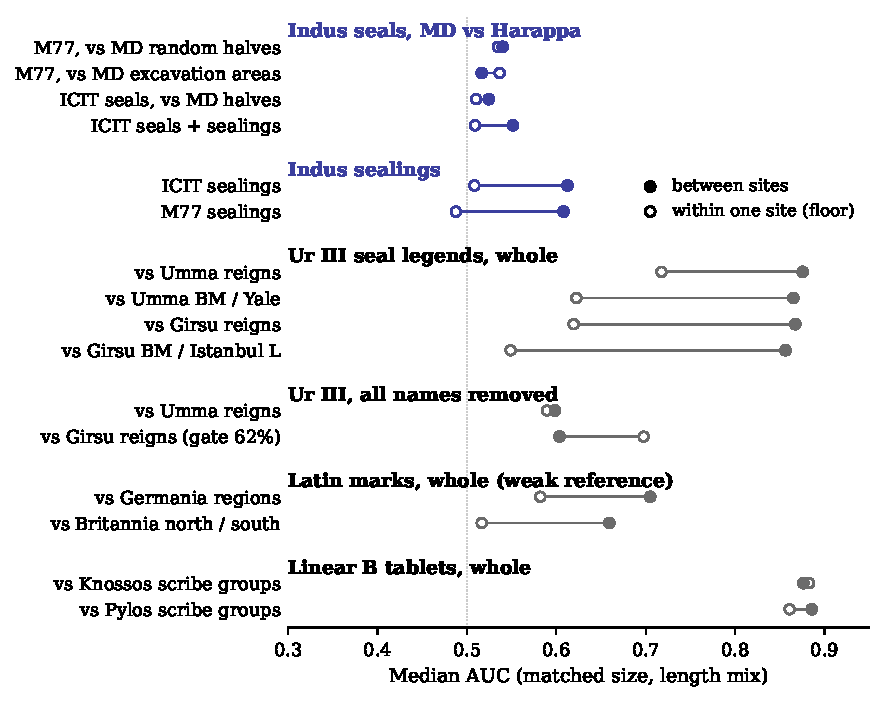
\includegraphics[width=0.82\textwidth]{fig1_between_within}
\caption{Between-site AUC (filled) against a within-site floor (open), at matched size and length mix. Indus rows in indigo. The Indus seal rows sit on their floors. Sealings do not. Whole Ur III and Latin legends sit well above their floors. Ur III with all names removed (step-2 tagging: proper-noun parts of speech, unknown forms and name determinatives) does not; Section~\ref{sec:names} and Table~\ref{tab:names} give the finer name-removal variants. Linear B scribe groups inside one palace separate as well as the two palaces. Sources: \texttt{experiments/uniformity\_paper/step2/results.json} and \texttt{experiments/redteam\_uniformity\_step1/results.json}; script \texttt{docs/paper/uniformity/figures/make\_fig1\_between\_within.py}.}
\label{fig:bw}
\end{figure}

\subsection{Readable seals carry place, much of it in personal names}
\label{sec:names}

The pipeline can see place when a seal corpus carries it.
Whole Ur III legends from Umma and Girsu score 0.86--0.88. % experiments/uniformity_paper/step2/RESULTS.md (Part 1)
Two reigns within one city score 0.62--0.72, and two museum collections 0.55--0.62. % S2
The gap above these floors is +0.16 to +0.31, and every gate passes. % S2
Random halves of one city give larger gaps (+0.36 and +0.40), but they are not a fair floor here. % S2 part1 U_rand +0.404, G_rand +0.355
Because the tablets came to museums in archive lots, the between-city contrast is also a between-archive contrast, and a reign or collection floor is the nearer match.
Counting each physical seal once (CDLI) gives the same pattern: +0.17 and +0.22 against the reign floors. % S2
So repeated impressions of one seal do not drive the result.
Latin owner and maker marks separate Britannia from Germania at 0.66--0.71, against 0.52--0.58 for two regions of one province: $\Delta$ = +0.12 and +0.14. % S2
Old Babylonian legends point the same way but are underpowered (gates 78\% and 56\%). % S2

Personal names carry much of the place signal in Ur III, but not all of it. % REVISION-PENDING: owner/father vs patron name split by legend slot (REVIEW_1 S1); patron names (governors, kings) are place markers by office
The third red team removed different kinds of names in turn (Table~\ref{tab:names}). % experiments/redteam_uniformity_step2/RESULTS.md (a)
With place names, divine names and every theophoric personal name removed, Umma against Girsu still clears all four within-city floors, by at least +0.102 (ORACC) and +0.093 (CDLI), with gates at 100\%. % RT2 (a)
So the signal is not a leak of city names or city gods such as \emph{umma}\textsuperscript{ki} or \v{S}ara.
With personal names removed but place names and gods kept, the gap falls below the strictest floor, two reigns of Girsu: $\Delta$ = +0.027 (ORACC, gate 86\%, $p_{\mathrm{floor}} = 0.137$) and +0.028 (CDLI, gate 92\%). % RT2 table.md (noPN G_reign)
It still clears the Umma reign floor, by +0.173 (ORACC, gate 98\%) and +0.123 (CDLI, gate 98\%). % RT2 table.md (noPN U_reign)
Against the two collection floors it is +0.159 and +0.174, but those gates (50\% and 78\%) fail. % RT2 table.md (noPN U_coll, G_coll)
On the Umma reign floor, the gap without personal names (+0.173) is larger than the gap without theophoric names (+0.102), so removing personal names does not erase place; it makes place indistinguishable from date in Girsu.
Whole legends drawn at the smaller name-free size still clear the reign floors by +0.164 (Umma, gate 90\%) and +0.213 (Girsu, gate 76\%), so pool size alone does not explain the drop. % RT2 table.md (wholeAtNF)
Many Ur III personal names are not private names in a simple sense.
On seals dedicated to a governor or king, the patron's name marks the province by office, and Umma and Girsu had their own governors.
We have not yet separated owners' names from patrons' names.

\begin{table}[t]
\centering
\small
\caption{Ur III Umma against Girsu: smallest and largest gap above the structural within-city floors whose power gate passes (80\%), by what is removed. ORACC has four structural floors (two reign, two collection), CDLI two (reign). From \texttt{experiments/redteam\_uniformity\_step2/table.md} (A1/A2) and \texttt{experiments/uniformity\_paper/step2/results.json}.}
\label{tab:names}
\begin{tabular}{lllll}
\toprule
 & \multicolumn{2}{l}{ORACC impressions} & \multicolumn{2}{l}{CDLI, one per seal} \\
Removed from the legends & smallest & largest & smallest & largest \\
\midrule
nothing (whole) & +0.158 & +0.307 & +0.165 & +0.222 \\ % S2 results.json part1 (whole: U_reign .158, G_coll .307; cdli U_reign .165, G_reign .222)
place names and gods & +0.137 & +0.280 & +0.126 & +0.189 \\ % RT2 table (noTG)
place names, gods, theophoric names & +0.102 & +0.267 & +0.093 & +0.195 \\ % RT2 table (noTGtheo)
personal names only & +0.027\rlap{$^a$} & +0.173 & +0.028\rlap{$^a$} & +0.123 \\ % RT2 table (noPN; ORACC collection floors gated out at 50%, 78%)
all names, strict tagging & +0.052\rlap{$^b$} & +0.052 & \multicolumn{2}{l}{underpowered} \\ % RT2 table (strict; only U_reign gated)
\bottomrule
\multicolumn{5}{l}{\footnotesize $^a$ Girsu reign floor; not above it ($p_{\mathrm{floor}} = 0.137$). $^b$ Only one split gated, at exactly 80\%; $p_{\mathrm{floor}} = 0.078$.}
\end{tabular}
\end{table}

Without personal names, place and date are hard to tell apart.
In step 2, name-free Umma against Girsu (0.599) was no higher than early against late reigns inside Umma (0.590): $\Delta$ = +0.009. % experiments/uniformity_paper/step2/RESULTS.md
Inside Girsu, the reign split (0.698) beat the between-city value (0.604), though that gate was 62\%. % S2
Stricter name tagging moved the Umma reign comparison to +0.052, exactly at the gate (80\%), and not significant against the floor ($p_{\mathrm{floor}} = 0.078$). % experiments/redteam_uniformity_step2/table.md (strict U_reign)
So the name-free comparison is a tie within about $\pm 0.05$: the gaps run from $-0.09$ to $+0.05$, depending on the floor and the tagging. % RT2 (safe wording) % REVISION-PENDING: "tie within +-0.05" is point-estimate wording; bootstrap CI + TOST (REVIEW_1 M3)
We do not claim that name-free legends carry no place.
The reign floors are high for a concrete reason.
In the Umma legends, royal-dedication seals of \v{S}ulgi and Amar-Suen call the king \emph{nita kal-ga} (368 legends, and 5 later ones), while those of \v{S}u-Suen and Ibbi-Suen write \emph{lugal kal-ga}. % RT2 (a, "Why the reign floors are high") % TODO: cite Frayne, RIME 3/2 for the royal epithets (REVIEW_1 B2.4, S10)
Name-free legends therefore carry a dated formula.

The Latin result needs a caveat on name tagging.
An audit of 50 kept and 50 removed tokens found the Ur III tagger sound (0\% and 4\% of kept tokens were names in ORACC and CDLI). % RT2 (audit table)
In Latin, 42\% of tokens kept as ``name-free'' were names or unclear, and 22\% of removed tokens were not names or unclear. % RT2 (audit table)
So we use only the whole Latin legends.
Without unit words and numerals, Britannia against Germania still clears both floors (+0.084 and +0.163). % RT2 (a)
We do not report a name-free Latin result.

\subsection{How many Indus seals could carry site-specific names}
\label{sec:bound}

If Indus seals named their owners the way Ur III seals do, the two cities should differ.
They do not.
The planted-names test turns this into a bound (Figure~\ref{fig:power}B).

In Ur III, 99.8\% of legends carry a personal name, at 1.86 names per legend and 36\% of tokens. % experiments/redteam_uniformity_step2/RESULTS.md (A3)
A name load like that is excluded in every Indus pool and every name form. % RT2 (A3)
% REVISION-PENDING: the grid jumps from r = 0.3 to 0.5, so "at most 30%" means "excluded at 50%, not at 30%"; rerun at r = 0, 0.35, 0.40, 0.45 with bootstrap variance (REVIEW_1 M2). This paragraph and the next wait on it.
Names spelt in shared signs with real Ur III frequencies are compatible with the observed gap on at most 30\% of seals, in all three pools. % RT2 (A3 table)
Invented name stocks are compatible on at most 10\% of seals, or 20\% for two-sign names in ICIT seals. % RT2 (A3 table)
Step 1, which used permuted labels and absolute AUC, gave 20--30\%. % experiments/uniformity_paper/step1/RESULTS.md and RT2 (A3)
Measured against the floor, the bound is tighter for invented stocks (10--20\%) and the same for realistic, overlapping names (30\%). % RT2 (A3)

Realistic names give the weaker bound for a simple reason.
Real name stocks overlap between cities, and many names are common.
A planted stock of this kind is harder to detect than an invented one.
The 30\% figure is therefore the one to quote.

\begin{figure}[t]
\centering
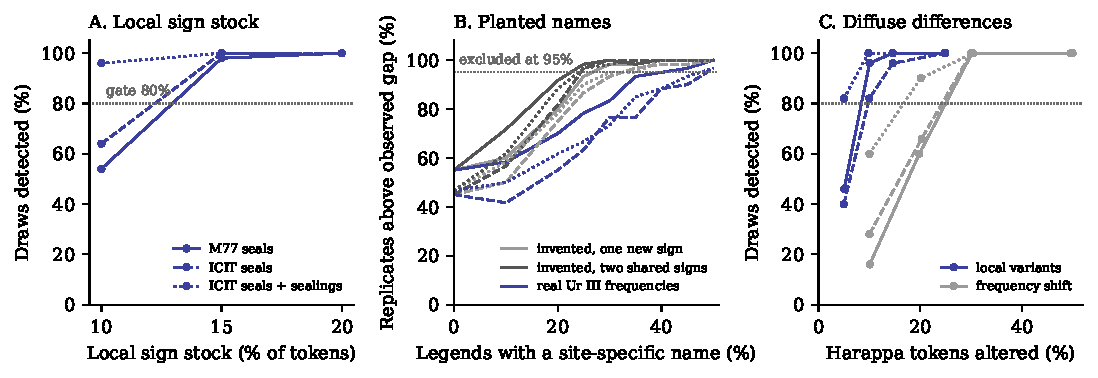
\includegraphics[width=\textwidth]{fig2_power}
\caption{Power. (A) Share of draws in which a 20-sign local stock planted on the Harappa side (seals, or seals and sealings in the third pool) at the given share of tokens is detected above the Mohenjo-daro floor; the gate is 80\% at 15\%. (B) Share of draws in which site-specific names on the given share of seals produce a larger gap than observed; a load is excluded at 95\%. Sources: \texttt{experiments/uniformity\_paper/step2/results.json} (A) and \texttt{experiments/redteam\_uniformity\_step2/results.json} (B); script \texttt{make\_fig2\_power.py}.}
\label{fig:power}
\end{figure}

\subsection{Limits of the tie}
\label{sec:limits}

\paragraph{Sealings differ.} Mohenjo-daro and Harappa sealings separate at 0.613 (ICIT) and 0.608 (M77): $\Delta$ = +0.104 and +0.120. % experiments/uniformity_paper/step2/RESULTS.md (Part 2)
The difference survives strict de-duplication (+0.091 and +0.167). % experiments/redteam_uniformity_step2/RESULTS.md (d)
This matters because Harappa sealings repeat heavily: in M77, 367 complete Harappa sealings carry 162 distinct strings, and one seal text is impressed 49 times. % RT2 (d)
We cannot say whether the sealing difference is place or format.
The test that compares each city's sealings with its own and the other city's seals is underpowered (gates 2--4\%). % RT2 (d)
Descriptively it leans towards format.
\citet[p.~19]{yadav2017} also singled out Harappa sealings.
We do not write that sealings show a place difference.

\paragraph{Tablets differ.} ICIT tablets separate at 0.774. % S2 (Part 2)
Most Mohenjo-daro ``tablets'' are copper tablets (197 of 299), while Harappa's are moulded or incised, so that number is not a place contrast. % S2
Moulded tablets alone still differ: $\Delta$ = +0.150, power 96\%. % RT2 (d)
Mohenjo-daro has only 42 moulded tablets, and Harappa's moulded tablets are a late series specific to that site. % RT2 (d)
A period or type difference within ``moulded'' is not excluded.

\paragraph{Chanhu-daro is a near-miss.} Chanhu-daro is the most separable site in every comparison with the two big cities (Figure~\ref{fig:sites}). % S2
A dedicated follow-up found that its seals sit +0.13 to +0.17 above both the within-site floor and the shuffled-label null, in two editions, with power of 96--98\%. % experiments/chanhudaro_followup/RESULTS.md (verdict, safe wording)
After correction, each of the four pairs has $q_{\mathrm{chance}} = 0.06$, so none clears the follow-up's bar of 0.05. % CD
Two rules apply here, and they disagree.
By the step-2 rule ($q_{\mathrm{floor}} \leq 0.10$ against the floor), Chanhu-daro ``differs'' from Harappa in both editions ($q_{\mathrm{floor}}$ = 0.098 in M77 seals, 0.074 in ICIT seals and sealings). % experiments/uniformity_paper/step2/results.json part2
The follow-up, written after step 2, asked for more: $q_{\mathrm{chance}} \leq 0.05$ against the shuffled-label null, which is the stricter reference because the small-pool floors sit below 0.5.
We let the stricter rule govern because it was the one written for this question, but it was set after the step-2 numbers were known. % docs/prereg/chanhudaro_followup.md L31-32
The four pairs share the same 40-odd Chanhu-daro seals, and the two editions overlap in objects, so they are not independent replications. % CD
We do not claim a Chanhu-daro place signal.

The follow-up ruled out several explanations.
Only 1 of 50 M77 Chanhu-daro seals lies at the Jhukar levels, and dropping it changes nothing. % CD (period); Mackay 1943: 143 says Jhukar seals carry no signs
Strict de-duplication enlarges the gap (+0.16 to +0.21). % CD
Dropping the 6 seals from one findspot (Square 9/D) leaves the M77 gaps at +0.13 to +0.14. % CD (T5; the ICIT rows are unchanged pools)
Restricting to unicorn seals leaves most of it in place. % CD (T4)
About half the gap comes from a few signs, mainly \sign{M93}. % CD
\sign{M93} is on 20\% of Chanhu-daro seals and ends 16\% of them. % CD (sign profile)
It is on none of 251 Harappa seals and none of 1,026 Mohenjo-daro seals in M77. % CD (sign profile)
Without these signs the gap falls to +0.06 to +0.08. % CD (safe wording)
\citet[pp.~145--149]{mackay1943} records local seal-making at Chanhu-daro and ``one new sign at least'' on its seals.
He does not mention an end mark.
The restriction of \sign{M93} to Chanhu-daro is not new information: all 11 of its occurrences in M77 are Chanhu-daro texts (10 seals and 1 sealing), so it can be read off the 1977 concordance, and 9 of them end the text or stand last. % data/m77_texts.jsonl (all M93 texts; 9 final, 2 medial); computed 2026-11-21, no new analysis run
ICIT does not have it as one sign: it writes two common signs, \sign{W031} \sign{W032}, a pair that occurs in that order 9 times at Chanhu-daro and once elsewhere, on a Kalibangan pot. % data/icit_texts.jsonl; experiments/toponyms/RESULTS.md item 4
What we have not seen discussed is its use as a local terminal mark and its weight in separating Chanhu-daro, but that rests on the sources we could read (Mackay 1943 and the open pages of Wells 2015); we have not read Wells 2011, Fuls's site-frequency work or Yadav 2013. % REVISION-PENDING: M93 novelty; check CISI photographs (ligature vs numeral pair) and the unread sources (REVIEW_1 M8, S3)
We excluded only the Jhukar period, not period in general: a depth split within Chanhu-daro has 17 seals per side and no power (gates 26\% and 16\%). % CD (T1b)

\paragraph{Smaller sites are underpowered or inconclusive.} No pair of Lothal, Kalibangan or Dholavira with Mohenjo-daro or Harappa reaches ``differs''. % S2
Power at $s = 0.15$ for those pairs runs from 48\% to 96\%. % experiments/uniformity_paper/step2/results.json part2 (power['0.15']); S2's summary line quotes the s = 0.10 column (16-84%)
Some fail the gate and are underpowered.
Others pass it with a gap above 0.05 and fail only on $q$, so they are inconclusive rather than underpowered: Harappa against Kalibangan in M77 ($\Delta$ = +0.125, power 96\%), Harappa against Dholavira in ICIT seals and sealings (+0.109, 92\%) and Harappa against Lothal in M77 (+0.068, 90\%). % results.json part2
Only Mohenjo-daro against Dholavira (ICIT seals and sealings) is gated ``same'' ($\Delta$ = +0.047). % S2
Pairs between two small sites have floors of 0.32--0.47, the pipeline's low bias on small pools. % S2 footnote; RT2 (c)
At a few dozen texts per side (19--37 for the small-site floors), these AUCs are uncertain by roughly $\pm 0.1$ or more, % S2 table footnote; REVIEW_1 B3 minor and the map in Figure~\ref{fig:sites} is for orientation only.
Every ``differs'' verdict among them flips to ``underpowered'' once the null is the reference. % RT2 (c)
So our result covers the two big cities.
It does not show that all Indus sites write alike.

\begin{figure}[t]
\centering
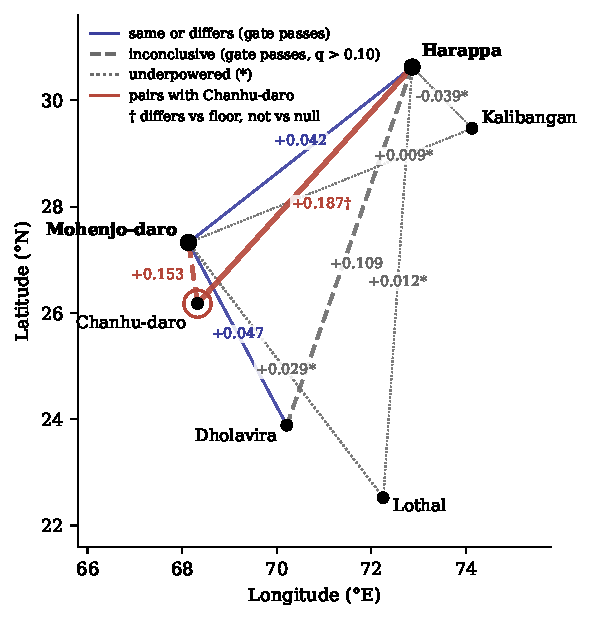
\includegraphics[width=0.62\textwidth]{fig3_sites}
\caption{Gap above the floor ($\Delta$, between $-$ within) for ICIT seals and sealings, for every pair with Mohenjo-daro or Harappa. Line width grows with $\Delta$. Solid lines are pairs whose power gate passes (``same'' or ``differs'' against the floor); dashed lines are gated but inconclusive ($\Delta \geq 0.05$, $q$ above 0.10); dotted lines with an asterisk fail the gate (underpowered). Harappa--Chanhu-daro ``differs'' against the floor only, not against the shuffled-label null (marked $\dagger$). Chanhu-daro is circled. Positions are approximate and for orientation only. Source: \texttt{experiments/uniformity\_paper/step2/results.json}; script \texttt{make\_fig3\_sites.py}.}
\label{fig:sites}
\end{figure}

\subsection{Reimplementing Recchia and Louwerse (2016)}
\label{sec:recchia}

\citet{recchia2016} report that LSA site vectors of Indus inscriptions recover the relative positions of five sites: Mohenjo-daro, Harappa, Chanhu-daro, Lothal and Kalibangan.
We could not read their full text.
The publisher returned a bot challenge to our client, and we did not try to get round it. % experiments/recchia_rerun/RESULTS.md (limits)
We reimplemented the method from the abstract: LSA with log-entropy weighting, summed site vectors, cosine distances, classical multidimensional scaling (MDS), and a Procrustes fit to site coordinates. % RR (safe wording)
We used M77 and treated seals and sealings separately.
Our seal set has 1,823 texts against their 1,936, and our sealing set 716 against their 723. % RR (limits)

The seal configuration was no closer to geography than chance.
The real site-to-coordinate assignment ranked 45th of 120 ($p = 0.38$), and the fit was below a site-label permutation null ($p = 0.61$). % RR (verdict, safe wording)
This held across dimensionality, vector normalisation, edition (ICIT) and near-duplicate removal. % RR (sensitivity table: the variant is unit-length document vectors, not another term weighting)
Sealing vectors differed between sites beyond the label null ($p = 0.025$) but not in a geographic arrangement ($p = 0.54$). % RR
This matches the sealing difference above.

The test is weak.
With five points, a planted geographic gradient affecting 15\% of seal tokens was detected in 30\% of simulations; seals reach 80\% only at 20\% of tokens. % RR (planted gradient table)
So we do not claim their result is false.
A real but modest geographic signal could have been missed.
It does not, however, rest on Mohenjo-daro and Harappa seals.
Their distance in the same LSA space lies at the edge of the within-Mohenjo-daro range: a median of 0.062 against a 95th percentile of 0.062, or 0.062 against 0.067 after near-duplicate removal. % RR (safe wording)
That is a narrow call: 48\% of the between draws exceed the within 95th percentile. % RR L24
Their settings may differ from ours, and their reported fit may come from a choice we did not try. % RR (limits)
% TODO: read Recchia & Louwerse 2016 full text before submission and check weighting, dimensions, MDS type and fit statistic.

\section{Discussion}
\label{sec:discussion}

\subsection{What the bound means}

The two big Indus cities share their seal vocabulary as closely as two halves of one city. % REVISION-PENDING: equivalence wording, bootstrap CI + TOST (REVIEW_1 M3)
In readable seal corpora that share does not hold, and personal names are a large part of the reason.
Ur III seals carry a personal name on almost every legend, with 1.86 names per legend on average. % experiments/redteam_uniformity_step2/RESULTS.md (A3: 99.8%, 1.86)
Names are local, so the city shows.

Indus seals do not show their city.
That leaves two readings that the data cannot yet separate.
First, Indus seals may name individuals, but from a shared pool of names used in both cities.
Names with no local preference would leave no place signal. % point made in experiments/uniformity_benchmark/RESULTS.md ("What this means")
Second, the seals may not name individuals at all.
They may record offices, titles, commodities or other terms common to the whole civilisation.
Either way, site-specific personal names cannot be on more than about 30\% of seals. % RT2 (A3) % REVISION-PENDING: finer planted-name grid (REVIEW_1 M2)

The second reading fits an earlier finding from this project, though that finding is itself not settled.
Seal-text cores, the non-frame part of a seal text, are mostly one or two word-signs, not syllabic spellings. % README.md finding #10; experiments/typology and experiments/core_semantics RESULTS
In that work, 34\% of cores were a single sign, and 80\% of signs in longer cores also stood alone as whole cores. % README.md finding #10
Its formal verdict was inconclusive (four of five pre-registered predictions passed), and it is the project's finding most sensitive to transcription: with noise matching the measured disagreement between the two editions it passes in only 3 to 9 of every 10 runs. % README.md finding #10 ("typology prereg 4/5 passed (formal verdict inconclusive)"; "passes in 3-9 of every 10 runs")
A spelled-out name system would look different.
That finding did not show that cores are not names, and neither does this one.
Together they make a site-specific, spelled personal name on most seals less likely, not ruled out.
Corpus statistics alone cannot say what the seals encode \citep{raghavendra2026}.

This also bears on the expectation that site-level analysis would revise the uniformity assumption \citep[p.~lvi]{kenoyer2010}.
For seal texts at Mohenjo-daro and Harappa, a site-level test with a floor does not revise it.
For sealings, tablets and Chanhu-daro, it leaves room for difference.
The regional variation in imagery and style documented by \citet{ameri2013}, \citet{jamison2017} and \citet{petrie2018} is outside this test.
Jamison's style groups cross sites, which is consistent with texts that do not follow the city.

\subsection{A methods lesson: the Linear B scribe trap}

Linear B shows what goes wrong without a floor.
Knossos and Pylos tablet lines separate at 0.904 at Indus size and length mix. % experiments/uniformity_paper/step1/RESULTS.md (A1)
That looks like strong place signal, and step 1 used it as one.
But groups of scribes inside one palace separate as strongly.
Knossos scribe groups score 0.883 against 0.876 between palaces at the same size; Pylos scribe groups score 0.861 against 0.886. % experiments/redteam_uniformity_step1/RESULTS.md
With series balanced and scribes held out of training, Knossos against Pylos falls to 0.524. % RT1 (attack 2)
The site classifier had learned scribes and offices, not palaces.
\citet[p.~296]{bennett1966} noted that Linear B handwriting is not uniform and follows individual scribes, and \citet{srivatsan2021} found hand and findplace entangled.

The lesson is general.
A site classifier on any script can learn excavation area, period, object type or scribe instead of place.
A between-site score means little until it is set against a within-site floor at the same size, together with a planted-difference power check.
Comparisons of scripts without such floors will tend to overstate place.
Mismatched designs can also mislead in the other direction. Our first benchmark compared an Indus value of 0.49 with references drawn in a different design; the like-for-like value was 0.55. % experiments/redteam_uniformity/RESULTS.md (0.49 not like-for-like; fair comparator 0.55)

\section{Limitations}
\label{sec:limitations}

\paragraph{Two cities, one object type.} The main result covers seals from Mohenjo-daro and Harappa.
Sealings and tablets differ between the two cities, Chanhu-daro is a near-miss, and comparisons with the smaller sites are underpowered or inconclusive.
The two editions overlap in objects, so they are two readings of largely one sample.

\paragraph{No interval on the gap.} $\Delta$ is a difference of two medians over subsampling draws from one finite pool, and the Harappa side is nearly the whole pool in every draw.
The spread across draws therefore understates sampling uncertainty, and ``same'' is a point-estimate rule, not an equivalence test. % REVIEW_1 B3.1-2; REVISION-PENDING: pool-level bootstrap CI and TOST (M3)

\paragraph{What the pre-registrations protected.} The Mohenjo-daro--Harappa number was known before every pre-registration; only the reference conditions, the later floors and nulls, the planted tests and the red-team attacks were blind.
The hash file is self-timestamped and became public with the results.
The Chanhu-daro bar was tightened after step 2 had been scored.
All eight runs took place within about one day.
None of this changes a number in this paper, but it limits how much protection the word ``pre-registered'' should be read to give.

\paragraph{A thin local stock could be missed.} A local stock covering 10\% of Harappa's tokens is found only about half the time. % experiments/redteam_uniformity_step1/RESULTS.md (attack 6)
Local carving variants that no published sign list records cannot be tested without sign images per site. % experiments/redteam_uniformity/RESULTS.md (attack 4)

\paragraph{Within-city floors are proxies.} The Mohenjo-daro area split mixes area with excavator and date: DK was dug by Mackay, HR and VS by Marshall's teams. % experiments/uniformity_paper/step1/RESULTS.md (caveats)
Half of the HR and VS seals have unconfirmed findspots. % RT1 (attack 4)
Ur III floors use reign and museum collection, because the catalogues record almost no excavation context. % S2
The Ur III between-city contrast is also between archives, which the Indus contrast is not.
The step-1 depth floor within Mohenjo-daro gives a gap of +0.09, above our margin; we discount it (Section~\ref{sec:tie}) but it is exploratory, not refuted.
Linear B floors use scribe groups, because no room or findspot data was available. % RT1 (limits)

\paragraph{The name-free comparison is a tie.} With all names removed, Ur III legends separate two cities about as well as two reigns of one city. % RT2 (safe wording) % REVISION-PENDING: tie wording, bootstrap (M3)
The verdict rests on one split whose gate is exactly 80\%. % RT2 (limits)
With only personal names removed, the gap still clears the Umma reign floor; it fails only against two reigns of Girsu. % RT2 table.md (noPN)
Latin name tagging is poor, so the Latin result is reported only for whole legends.

\paragraph{Different units.} The readable references are written in words, Indus in signs.
A word may carry more site information than a sign.
Splitting Linear B words into syllabic signs still gave 0.86, so the unit alone does not erase site signal. % experiments/uniformity_paper/step1/RESULTS.md (A9)
That check was on a reference later shown to carry scribe rather than place signal.

\paragraph{Few references.} The contrast rests on two readable seal corpora, Ur III and Latin, and few city pairs.
Old Babylonian was underpowered. % S2
Whether other name-bearing seal corpora behave like Ur III is untested.

\paragraph{Statistical floor.} With 50 draws per condition, the smallest possible $p$ is 0.020, which limits how small $q$ can get in families of 10--15 pairs. % experiments/redteam_uniformity_step2/RESULTS.md (limits)

\paragraph{Literature not yet read.} We could not read \citet{recchia2016} in full: the publisher's free copy refused our automated client, and no repository copy was found. % LITERATURE.md sec. 9 (2026-11-21: Wiley pdfdirect 403; Tilburg portal has no file)
Two directly relevant studies were also not read: Yadav's earlier work on how Indus signs vary with site and object type \citep{yadav2013}, and a chapter on toponyms in the script \citep{mahadevan2018}. % Open copies are listed on harappa.com, which blocks automated clients (Cloudflare); not circumvented. TODO: read both before submission.
Nor have we read \citet{wells2011}, which \citet{wells2015} cites for site and object differences in sign inventories.

\paragraph{Analysis by AI agents.} Most analyses and all red teams were carried out by AI agents working under written rules, with a human lead who set the questions and reviewed the findings.
Pre-registration and hashing limit what an agent could adjust after seeing data, within the bounds described above.
The attacking agents share a model family with the original analysts, so their independence is partial, and none of this replaces review by epigraphers and Assyriologists.

\section*{Data and code availability}
\label{sec:availability}

Code, pre-registrations with their hashes, results files and a ledger of every test run are available in the project repository (URL withheld for anonymous review; given in the named submission copy).
Corpus construction and editions follow \citet{openindus2026corpus}.
The experiments are in \nolinkurl{experiments/uniformity_benchmark/}, \nolinkurl{experiments/redteam_uniformity/}, \nolinkurl{experiments/uniformity_paper/step1/}, \nolinkurl{experiments/redteam_uniformity_step1/}, \nolinkurl{experiments/uniformity_paper/step2/}, \nolinkurl{experiments/redteam_uniformity_step2/}, \nolinkurl{experiments/chanhudaro_followup/} and \nolinkurl{experiments/recchia_rerun/}.
Each folder holds a \nolinkurl{RESULTS.md}, a \nolinkurl{results.json}, per-draw values and ledger rows.
The pre-registrations are in \nolinkurl{docs/prereg/} under the same names.
Their SHA-256 hashes, with the code they froze, are in \nolinkurl{docs/prereg/HASHES.txt} under the tags \nolinkurl{uniformity_benchmark}, \nolinkurl{redteam_uniformity}, \nolinkurl{uniformity_paper_step1}, \nolinkurl{redteam_uniformity_step1}, \nolinkurl{uniformity_paper_step2}, \nolinkurl{redteam_uniformity_step2}, \nolinkurl{chanhudaro_followup}, \nolinkurl{chanhudaro_followup_deviation1} and \nolinkurl{recchia_rerun}.
The figures are made by the scripts in \nolinkurl{docs/paper/uniformity/figures/}, which read the \nolinkurl{results.json} files directly.
Third-party texts (Indus editions, ORACC, CDLI, EDH, DAMOS) are not redistributed; scripts rebuild the pools from the public sources.

\section*{Use of AI}

AI agents performed most analyses, red teams and drafting, as described under Limitations.
The human author set the research questions and directed and reviewed the work.
Reported numbers were checked against their results files by agent review.

\section*{Competing interests and funding}

None declared. The work received no external funding.

\bibliographystyle{plainnat}
\bibliography{refs}

\end{document}
